\begin{figure*}
\resizebox{\textwidth}{!}{
\begin{tabular}{cccc}
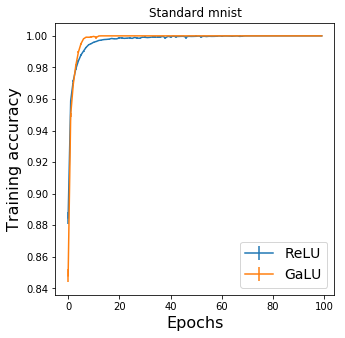
\includegraphics[scale=0.1]{figs/mnist-normal-opt.png}
&
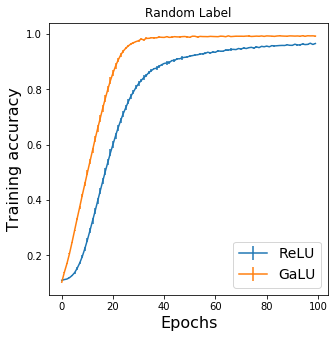
\includegraphics[scale=0.1]{figs/mnist-rand-label.png}
&
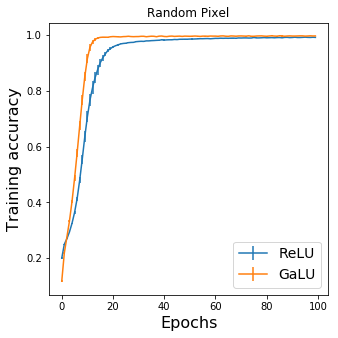
\includegraphics[scale=0.1]{figs/mnist-rand-pixel.png}
&
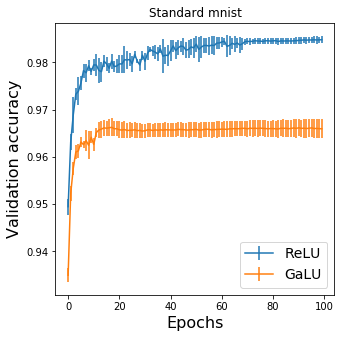
\includegraphics[scale=0.1]{figs/mnist-normal-gen.png}
	\end{tabular}
}
\caption{First three plots from the left show optimisation in ReLU and GaLU networks for standard MNIST, MNIST with random label and pixels  The right most plot shows generalisation of ReLU and GaLU networks in standard MNIST. Architecture we use is $d=7$, with layer widths from the first to last given by $512,512,256,256,128,64,10$ followed by a soft-max layer. In the case of GaLU there are two such network, wherein, one network is used to generate the gating values (whose weights are frozen) and the other network has the weights that are trained.}
\label{fig:galu-relu}
\end{figure*}
